\section{View}

Es wurde eine View mittels Spring MVC erstellt. Anstatt xHTML wie in JSF wird hier Thymeleaf verwendet. Dieses Framework erlaubt es Daten von POJOs als Inhalt anzuzeigen.

\subsection{Funktionsweise}

\begin{code}[]{java}
	 @GetMapping(value="/admin")
	public ModelAndView admin(){
		ModelAndView modelAndView = new ModelAndView();
		
\end{code}

Wenn eine Seite geladen wird, wird ein ModelAndView Objekt zurückgeliefert, welches von Thymleafe verarbeitet wird.

\begin{code}[]{java}
	modelAndView.setViewName("admin");
\end{code}


Mit setViewName wird der Name des Templates gesetzt, welches die Daten verarbeitet.

\begin{code}[]{java}

	List<Benutzer> benutzer = userService.getAll();
	
	System.out.println(benutzer.size());
	
	modelAndView.addObject("benutzers",benutzer);
	modelAndView.addObject("benutzer",new Benutzer());
	
	return modelAndView;
	}
\end{code}

Die Daten werden als Key-Value Paar gesetzt und können dann in Thymeleaf mit dem key verwendet werden.
\begin{code}[]{html}
	
	<tr th:each="Benutzer : \${benutzers}">
	<th scope="row" th:text="\${Benutzer.ID}"></th>
	<td th:text="\${Benutzer.vorName}"></td>
	<td th:text="\${Benutzer.nachName}"></td>
\end{code}

In der HTML Seite kann das Model mittels th: verwendet werden. th:each erstellt den Tag für jedes objekt in der Liste ''benutzers'' und nimmt als iterator referenz ''Benutzer''. Von diesen Elementen können die Attribute wie in Java abgefragt und eingefügt werden.

\clearpage

\begin{code}[]{html}
	
	<form class="form-inline" action="#" th:action="@{/admin}" th:object="\${benutzer}" method="post" >
	
\end{code}

Formulare können ebenfalls mit Thymeleaf in ein JSON Objekt gepackt und an den Server geschickt werden. Hierfür muss im Model ein leeres Objekt beigefügt sein.


\begin{code}[]{html}

<td><input class="form-control" type="text" th:field="*{vorName}" th:value="Vorname"/></td>
<td><input class="form-control" type="text" th:field="*{nachName}" th:value="Nachname"/></td>
\end{code}

Die einzelnen Attribute können mit th:field gemapped werden.


\begin{code}[]{java}
	@PostMapping(value = "/admin",produces = "application/json", consumes = MediaType.APPLICATION_JSON_VALUE)
	public ModelAndView adminAddUser(@RequestBody Benutzer b){
		userService.saveUser(b);
		
		return admin();
	}
\end{code}

Im Controller wird die POST Request mit einem Benutzer JSON im Request Body erwartet und geparsed.

\section{User managment}

Für das User managment wurde Spring Security verwendet.

\begin{code}[]{java}
@Override
public void configure(WebSecurity web) throws Exception{
	web.ignoring()
	.antMatchers("/resources/**","/static/**","/css/**","/js/**","/images/**");
}
\end{code}

Mit Spring Security werden generell alle Resource gesperrt. Damit man auf die statischen Inhalte zugreifen kann, werden diese von Spring Security auf ignore gesetzt.

\begin{code}[]{java}
	@Override
	protected void configure(HttpSecurity http) throws Exception {
		http.authorizeRequests()
		.antMatchers("/login").permitAll()
		.antMatchers("/registration").permitAll()
		.antMatchers("/index").authenticated()
		.and().csrf().disable().formLogin()
		.loginPage("/login").failureUrl("/login?error=true")
		.defaultSuccessUrl("/")
		.usernameParameter("email")
		.passwordParameter("password")
		.and().logout()
		.logoutRequestMatcher(new AntPathRequestMatcher("/logout"))
		.logoutSuccessUrl("/").and().exceptionHandling();
	}
\end{code}
 
Die Einzelnen Seiten können entweder ohne einschränkung oder mit authentifizierung festgelegt werden. Damit die Benutzer mit den richtigen Attributen authentifiziert werden, müssen diese Festgelegt werden. In diesem fall ''.usernameParameter("email")'' und ''.passwordParameter("password")''.

\begin{code}[]{java}
	@Autowired
	private BCryptPasswordEncoder bCrypt;
	
	 @Value("\${spring.queries.users-query}")
	private String userQuery;
	
	@Value("\${spring.queries.roles-query}")
	private String roleQuery;
	
	@Override
	protected void configure(AuthenticationManagerBuilder auth) throws Exception{
		auth.jdbcAuthentication()
		.usersByUsernameQuery(userQuery)
		.authoritiesByUsernameQuery(roleQuery)
		.dataSource(dataSource)
		.passwordEncoder(bCrypt);
	}
\end{code}

Damit die richtigen Attribute abgefragt werden müssen die Queries gesetz werden und der Verschlüsselungsalgorithmus für das Passwort.

\begin{code}[]{java}

	spring.queries.users-query=select e_mail as username, passwort as password, active as enabled from Benutzer where e_mail=?
	spring.queries.roles-query=select e_mail as username, 'default' from Benutzer where e_mail=?
	
\end{code}

Die Queries werden in HQL mit einem Parameter in application.properties festgelegt.

\section{Deployment}

Die Applikation wurde auf Heroku deployed.

\begin{figure}
	\centering
	
\includegraphics[width=0.7\linewidth]{images/screenshot001}
	\caption{Dashboard}
	\label{fig:screenshot001}
\end{figure}

In der Applikationsübersicht kann über den ''New'' Button eine neue Applikation hinzugefügt werden.

\begin{figure}
	\centering
	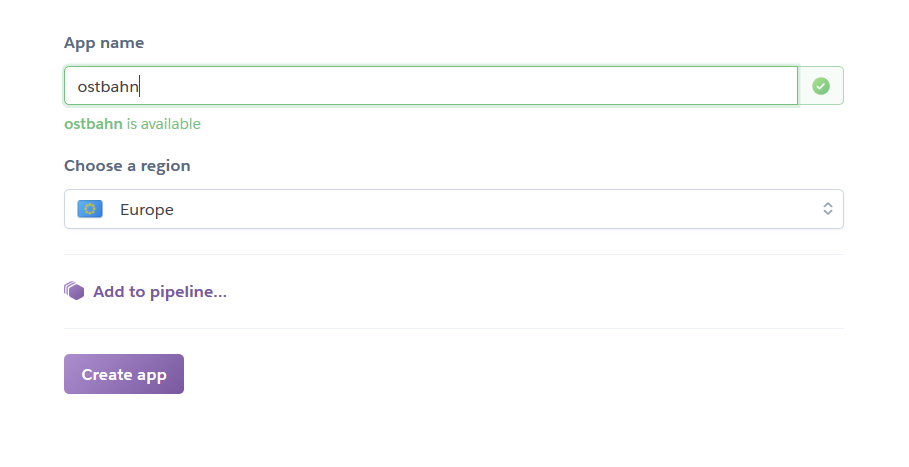
\includegraphics[width=0.7\linewidth]{images/screenshot002}
	\caption{Erstellen Dialog}
	\label{fig:screenshot002}
\end{figure}

In dem Dialog muss der Name hinzugefügt werden. Dort kann auch die Server position gewählt werden, welche auf Europa gesetz wurde.

\begin{figure}
	\centering
	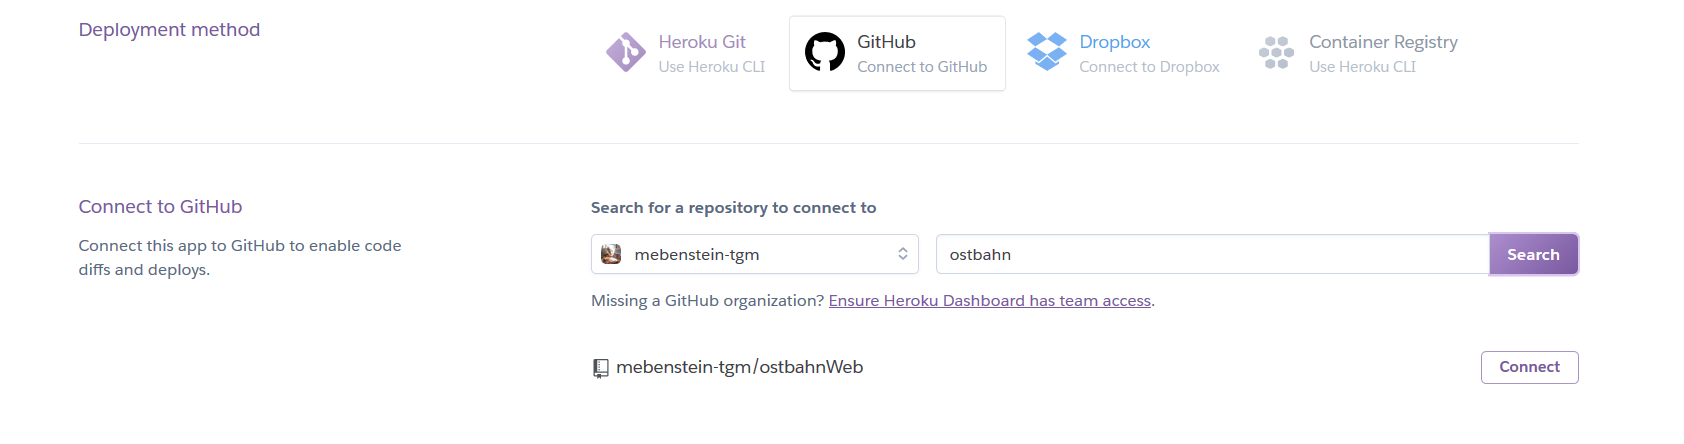
\includegraphics[width=0.7\linewidth]{images/screenshot004}
	\caption{Github connection}
	\label{fig:screenshot004}
\end{figure}

Um die Applikation zu deployen wird diese mit dem Github repository verbunden. Dafür wird das entsprechende Repository ausgewählt.\\

\begin{figure}
	\centering
	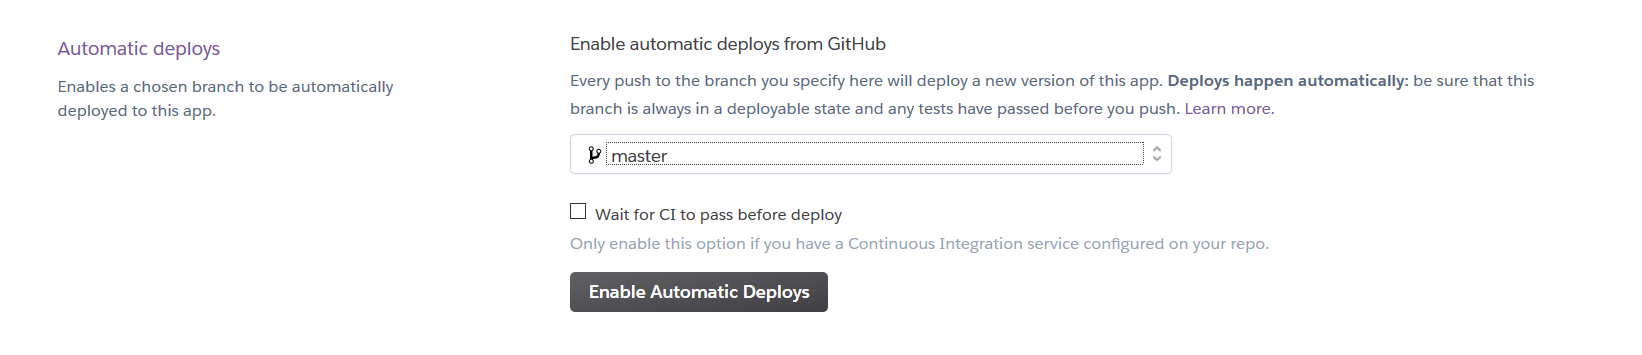
\includegraphics[width=0.7\linewidth]{images/screenshot005}
	\caption{Automatic Deployment}
	\label{fig:screenshot005}
\end{figure}

Mit dieser Konfiguration kann eingestellt werden, dass bei jedem Push die Applikation neu deployed wird.

